\documentclass{jsarticle}
\usepackage{amsmath,amssymb}
\usepackage[dvipdfmx]{graphicx}

\usepackage{tikz}
\usepackage{circuitikz}
\usetikzlibrary{arrows,shapes.gates.logic.US,shapes.gates.logic.IEC,calc}
\usetikzlibrary{shapes.geometric, positioning, calc} % ripple-carry-adder用重複気になる人は適当に削ってください。
\begin{document}

以下に使いそうな図を載せます。適当に使ってください。

剽窃判定怖いので、\textbf{コピペする場合は引用付けてほしい}ですが、ちょっといじった場合でも参考文献でつけてくれたら神様!ってなります。

レポートのサイズと部品のサイズが合わない場合は(ほとんどがそうだと思いますが、\textbackslash scalebox\{1\}の1を好きな倍率に変えてください。)


%---以下FF------------------------------------------------
\tikzset{ff/.style={flipflop, flipflop def={
          t1={D}, t2={}, c3=1, t4={},t5={},t6={Q},clock wedge size=.3, nd=0}},
}

\begin{figure}[h]
  \begin{center}
    \scalebox{1}{ % <-- ココで倍率調整
      \begin{tikzpicture}
        \node[ff](FF1){FF};
        \node[not gate US, draw, rotate=180] at ($(FF1.pin 1)!0.5!(FF1.pin 6)+(0,1)$) (Not) {};
        \draw (FF1.pin 1) -- ++ (-0.15,0)
        to[short]++(0,1);
        \draw (FF1.pin 6) -- ++ (0.15,0)
        to[short]++(0,1)
        to[short](Not.input);
        \draw (Not.output)
        to[short]($(FF1.pin 1) + (-0.15,1)$);
        \draw($(FF1.down)$)
        to[short,a=rst]++(0,-0.1);
        \draw($(FF1.pin 3)$)
        to[short,a=clk]++(-0.15,0);
        \draw($(FF1.down)$)
        to[short]++(0,0.29);
      \end{tikzpicture}
    }
  \end{center}
  \caption{flipflop}
\end{figure}

%---以下Latch------------------------------------------------
\tikzset{latch/.style={flipflop, flipflop def={
          t1={D}, t2={}, t3={clk}, t4={},t5={},t6={Q}, nu=0}},
}

\begin{figure}[h]
  \begin{center}
    \scalebox{1}{ % <-- ココで倍率調整
      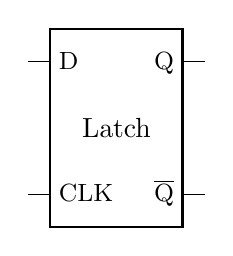
\begin{tikzpicture}
        \node[latch]{Latch};
      \end{tikzpicture}
    }
  \end{center}
  \caption{latch}
\end{figure}



%---以下Hulladder------------------------------------------------
\tikzset{halfadder/.style={flipflop,scale=.8, flipflop def={
          t1={inA}, t2={}, t3={inB}, t4={C},t5={},t6={S}, nu=0}},
}
\begin{figure}[h]
  \begin{center}
    \scalebox{1}{ % <-- ココで倍率調整
      \begin{tikzpicture}[]
        \node[halfadder] at (0,0)(halfadder1){halfadder};
        \node[halfadder] at (2.5,-3)(halfadder2){halfadder};
        \node[or gate US, draw, rotate=0,scale=2.2] at (5,-1.5)(or){};

        \node (inA) at ($(halfadder1.pin 1) + (-0.4,0)$) {inA};
        \node (inB) at ($(halfadder1.pin 3) + (-0.4,0)$) {inB};
        \node (cin) at (inB |- halfadder2.pin 4) {cin};
        \node (c) at ($(or.output)+(0.6,0)$) {c};
        \node (s) at (c |- inA) {s};

        %haisen      
        \draw (or.input 2) -- ++ (-0.5,0)
        |- (halfadder2.pin 4);
        \draw (or.input 1) -- ++ (-0.5,0)
        |- (halfadder1.pin 4);

        \draw (cin) -- (halfadder2.pin 3);
        \draw (halfadder1.pin 6) -- ++ (0.3,0)
        |- (halfadder2.pin 1);
        \draw (halfadder2.pin 6) -- ++ (0.1,0)
        |- (s);
        \draw (or.output) -- (c);
      \end{tikzpicture}
    }
    \caption{fulladder}
  \end{center}
\end{figure}


%---以下4bit-Ripple-Carry-Adder------------------------------------------------
\begin{figure}[h]
  \begin{center}
    \scalebox{1}{ % <-- ココで倍率調整
      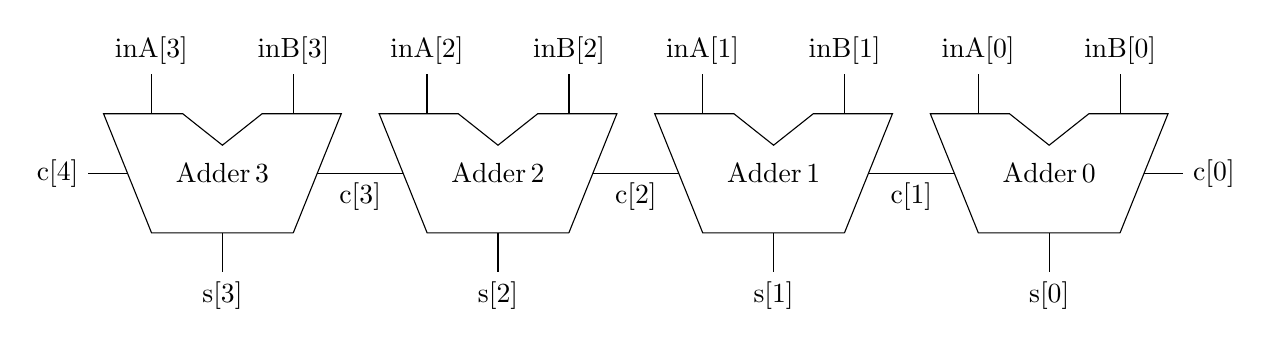
\begin{tikzpicture}[%
          alu/.style={trapezium,
              trapezium angle=45,
              shape border rotate=180,
              minimum width=3cm,
              minimum height=1.5cm,
              trapezium stretches=true,
              append after command={%
                  \pgfextra
                  \draw (\tikzlastnode.top left corner) --
                  (\tikzlastnode.top right corner) --
                  (\tikzlastnode.bottom right corner) --
                  ($(\tikzlastnode.bottom right corner)!.666!(\tikzlastnode.bottom side)$)--
                  ([yshift=-4mm]\tikzlastnode.bottom side)--
                  ($(\tikzlastnode.bottom side)!.334!(\tikzlastnode.bottom left corner)$)--
                  (\tikzlastnode.bottom left corner)--
                  (\tikzlastnode.top left corner);
                  \endpgfextra}},
        ]

        \node[alu] (alu3) at(0,0) {Adder\,3};
        \node[alu] (alu2) at(3.5,0) {Adder\,2};
        \node[alu] (alu1) at(7,0) {Adder\,1};
        \node[alu] (alu0) at(10.5,0) {Adder\,0};

        \draw (alu0.south) -- ++(-90:5mm) node [below] (out) {s[0]};
        \draw (alu0.0) -- ++(0:5mm) node  [right] {c[0]};
        \draw (alu0.40) -- ++(90:5mm) node [above] {inB[0]};
        \draw (alu0.140) -- ++(90:5mm) node [above] {inA[0]};

        \draw (alu1.south) -- ++(-90:5mm) node [below] (out) {s[1]};
        \draw (alu1.40) -- ++(90:5mm) node [above] {inB[1]};
        \draw (alu1.140) -- ++(90:5mm) node [above] {inA[1]};

        \draw (alu2.south) -- ++(-90:5mm) node [below] (out) {s[2]};
        \draw (alu2.40) -- ++(90:5mm) node [above] {inB[2]};
        \draw (alu2.140) -- ++(90:5mm) node [above] {inA[2]};

        \draw (alu3.south) -- ++(-90:5mm) node [below] (out) {s[3]};
        \draw (alu3.40) -- ++(90:5mm) node [above] {inB[3]};
        \draw (alu3.140) -- ++(90:5mm) node [above] {inA[3]};
        \draw (alu3.180) -- ++(0:-5mm) node [left] {c[4]};

        \draw (alu0.180) --  node [below]{c[1]}(alu1.0);
        \draw (alu1.180) --  node [below]{c[2]}(alu2.0);
        \draw (alu2.180) --  node [below]{c[3]}(alu3.0);
      \end{tikzpicture}
    }
  \end{center}
  \caption{4bit-ripple-carry-adder}
\end{figure}


\end{document}
